\chapter{Giới thiệu}
\label{ch:gioi-thieu}

\section{Bối cảnh và vấn đề nghiên cứu}
\label{sec:boi-canh}

Rối loạn trầm cảm (Major Depressive Disorder) là một trong những nguyên nhân hàng đầu gây suy giảm chất lượng cuộc sống và gia tăng gánh nặng y tế cộng đồng trên phạm vi toàn cầu \cite{pratt2014depression}. Theo Tổ chức Y tế Thế giới, hàng trăm triệu người thuộc nhiều lứa tuổi đang phải đối mặt với các mức độ triệu chứng trầm cảm khác nhau. Không chỉ ảnh hưởng tiêu cực đến sức khỏe tinh thần, năng suất lao động và gắn kết gia đình, trầm cảm mức độ nặng còn liên quan mật thiết đến nguy cơ tự tử. Đáng chú ý, nhiều người có triệu chứng ở giai đoạn đầu hoặc mức độ nhẹ thường không nhận biết được tình trạng của mình, hoặc e ngại rào cản tâm lý xã hội, dẫn đến việc chậm trễ tiếp cận các dịch vụ hỗ trợ y tế.

Trong thực hành lâm sàng và các nghiên cứu dịch tễ học, công cụ phổ biến nhất để sàng lọc và đánh giá mức độ triệu chứng trầm cảm là Thang đo Sức khỏe Bệnh nhân 9 mục (Patient Health Questionnaire-9 -- PHQ-9) do Kroenke và cộng sự phát triển \cite{kroenke2001phq, spitzer1999validation}. PHQ-9 gồm 9 câu hỏi tự điền tương ứng với các tiêu chuẩn triệu chứng trong Sổ tay Chẩn đoán và Thống kê Rối loạn Tâm thần (DSM-IV). Mỗi câu hỏi được tính từ 0 đến 3 điểm, tạo nên tổng điểm dao động từ 0 đến 27 điểm. Trong y văn, thang điểm này thường được chia thành năm khoảng mức độ: Tối thiểu (0--4 điểm), Nhẹ (5--9 điểm), Vừa (10--14 điểm), Nặng vừa (15--19 điểm) và Nặng (20--27 điểm).

Mặc dù PHQ-9 có độ tin cậy sàng lọc cao, phương pháp này vẫn phụ thuộc vào bản chất tự báo cáo của người tham gia khảo sát. Người điền bảng hỏi có thể khai báo chưa đầy đủ hoặc không nhất quán do tâm lý chủ quan hay định kiến cá nhân. Vì vậy, việc tìm hiểu khả năng khai thác các chỉ số khách quan từ hồ sơ kiểm tra sức khỏe thể chất và xét nghiệm cận lâm sàng dạng bảng để hỗ trợ sàng lọc mức độ triệu chứng là một hướng nghiên cứu đáng quan tâm trong y tế dự phòng và chăm sóc sức khỏe ban đầu.

Các cuộc điều tra sức khỏe quy mô dân số, tiêu biểu là Khảo sát Sức khỏe và Dinh dưỡng Quốc gia Hoa Kỳ (NHANES) do CDC thực hiện định kỳ hai năm một lần \cite{cdc2014nhanes, cdc2016nhanes}, cung cấp nguồn dữ liệu dạng bảng phong phú. NHANES kết hợp phỏng vấn nhân khẩu, thăm khám thể lực và các xét nghiệm sinh hóa máu chuẩn hóa. Một số nghiên cứu y sinh học đã ghi nhận mối liên hệ gián tiếp giữa triệu chứng trầm cảm và các chỉ số chuyển hóa toàn thân, bao gồm phản ứng viêm thể nhẹ, nồng độ lipid máu, huyết áp và chỉ số khối cơ thể.

Học máy là công cụ phù hợp để tìm kiếm các mối quan hệ phi tuyến giữa các chỉ số sinh lý đa biến. Tuy nhiên, khi áp dụng các thuật toán học máy vào bài toán dự đoán mức độ triệu chứng PHQ-9 trên dữ liệu khảo sát cộng đồng dạng bảng, mô hình phải đối mặt với ba thách thức kỹ thuật lớn:
\begin{enumerate}
    \item \textit{Mất cân bằng lớp cực đoan:} Trong quần thể dân cư nói chung, phần lớn người tham gia khảo sát thuộc nhóm triệu chứng tối thiểu (chiếm khoảng 74--76\%), trong khi nhóm có triệu chứng nặng chỉ chiếm khoảng 1.0--1.3\%. Sự chênh lệch này khiến các mô hình học máy thông thường có xu hướng dự đoán nghiêng về lớp đa số để đạt độ chính xác tổng thể cao nhưng bỏ sót các ca có triệu chứng thực tế.
    \item \textit{Chồng lấn phân phối đặc trưng:} Khác với các bệnh lý có chỉ dấu sinh học đặc hiệu trong máu, các chỉ số sinh lý ngoại vi giữa người có triệu chứng tối thiểu và người có triệu chứng nhẹ phân tán rộng và chồng lấn đáng kể. Ranh giới phân tách trong không gian đặc trưng trở nên mờ nhạt, khiến các mô hình phân loại phẳng dễ nhầm lẫn giữa các mức độ kế cận.
    \item \textit{Suy giảm hiệu năng theo độ chi tiết nhãn:} Phần lớn các công trình trước đây tập trung vào bài toán phân loại nhị phân (Không có triệu chứng so với Có triệu chứng). Khi mở rộng bài toán sang phân loại đa mức để phục vụ phân tầng chi tiết hơn, hiệu năng của các thuật toán học máy giảm rõ rệt.
\end{enumerate}

Xuất phát từ các vấn đề thực tế trên, đề tài nghiên cứu khung học máy cho dự đoán mức độ triệu chứng trầm cảm từ dữ liệu sinh lý được thực hiện nhằm xây dựng, thử nghiệm và đánh giá có hệ thống khung thực nghiệm DepSev-ML. Nghiên cứu tập trung khảo sát và so sánh nhiều hướng tiếp cận học máy khác nhau trên dữ liệu dạng bảng NHANES, nhằm tìm hiểu hiệu quả, đặc điểm phân loại và sự đánh đổi giữa các chỉ số đánh giá trong dự đoán mức độ triệu chứng trầm cảm. Cần lưu ý rằng, nghiên cứu này không hướng tới việc thay thế bảng câu hỏi PHQ-9 hay đưa ra chẩn đoán lâm sàng tự động thay bác sĩ tâm thần, mà tập trung làm rõ tiềm năng và giới hạn thực nghiệm của các đặc trưng sinh lý ngoại vi trong các bài toán phân loại đa mức.

\section{Phát biểu bài toán}
\label{sec:phat-bieu-bai-toan}

Xét một tập dữ liệu y tế dạng bảng gồm $N$ đối tượng khảo sát:
\begin{equation}
    \mathcal{D} = \left\{ (\mathbf{x}_i, s_i) \right\}_{i=1}^N
\end{equation}
trong đó $\mathbf{x}_i \in \mathbb{R}^d$ là vectơ $d$ đặc trưng dạng bảng đại diện cho đối tượng thứ $i$, bao gồm các biến nhân khẩu học, chỉ số nhân trắc, huyết áp, các xét nghiệm sinh hóa máu và thói quen lối sống; $s_i \in \{0, 1, \dots, 27\}$ là tổng điểm PHQ-9 tự báo cáo của đối tượng đó.

Điểm số $s_i$ được ánh xạ thành nhãn phân loại rời rạc $y_i \in \{0, 1, \dots, K-1\}$ thông qua hàm phân khoảng $g_K: \{0, \dots, 27\} \to \{0, \dots, K-1\}$. Để tìm hiểu đặc điểm dữ liệu ở các độ phân giải khác nhau, nghiên cứu thiết lập hai không gian mục tiêu chính:
\begin{itemize}
    \item \textit{Bài toán 5 mức độ tiêu chuẩn ($T_5$):} $K = 5$, tương ứng với 5 khoảng điểm PHQ-9 chuẩn trong y văn: Tối thiểu ($C_0: 0 \le s \le 4$), Nhẹ ($C_1: 5 \le s \le 9$), Vừa ($C_2: 10 \le s \le 14$), Nặng vừa ($C_3: 15 \le s \le 19$), và Nặng ($C_4: 20 \le s \le 27$).
    \item \textit{Bài toán 3 nhóm theo quy ước lâm sàng ($T_3$):} $K = 3$, gom các mức từ vừa đến nặng thành một nhóm để phục vụ định hướng hành động y tế dự phòng: Tối thiểu ($C_0: 0 \le s \le 4$), Nhẹ ($C_1: 5 \le s \le 9$), và Nặng theo quy ước ($C_2^+: s \ge 10$).
\end{itemize}

\begin{figure}[htbp]{Mô hình hóa bài toán dự đoán mức độ triệu chứng trầm cảm từ dữ liệu sinh lý dạng bảng.}
\centering
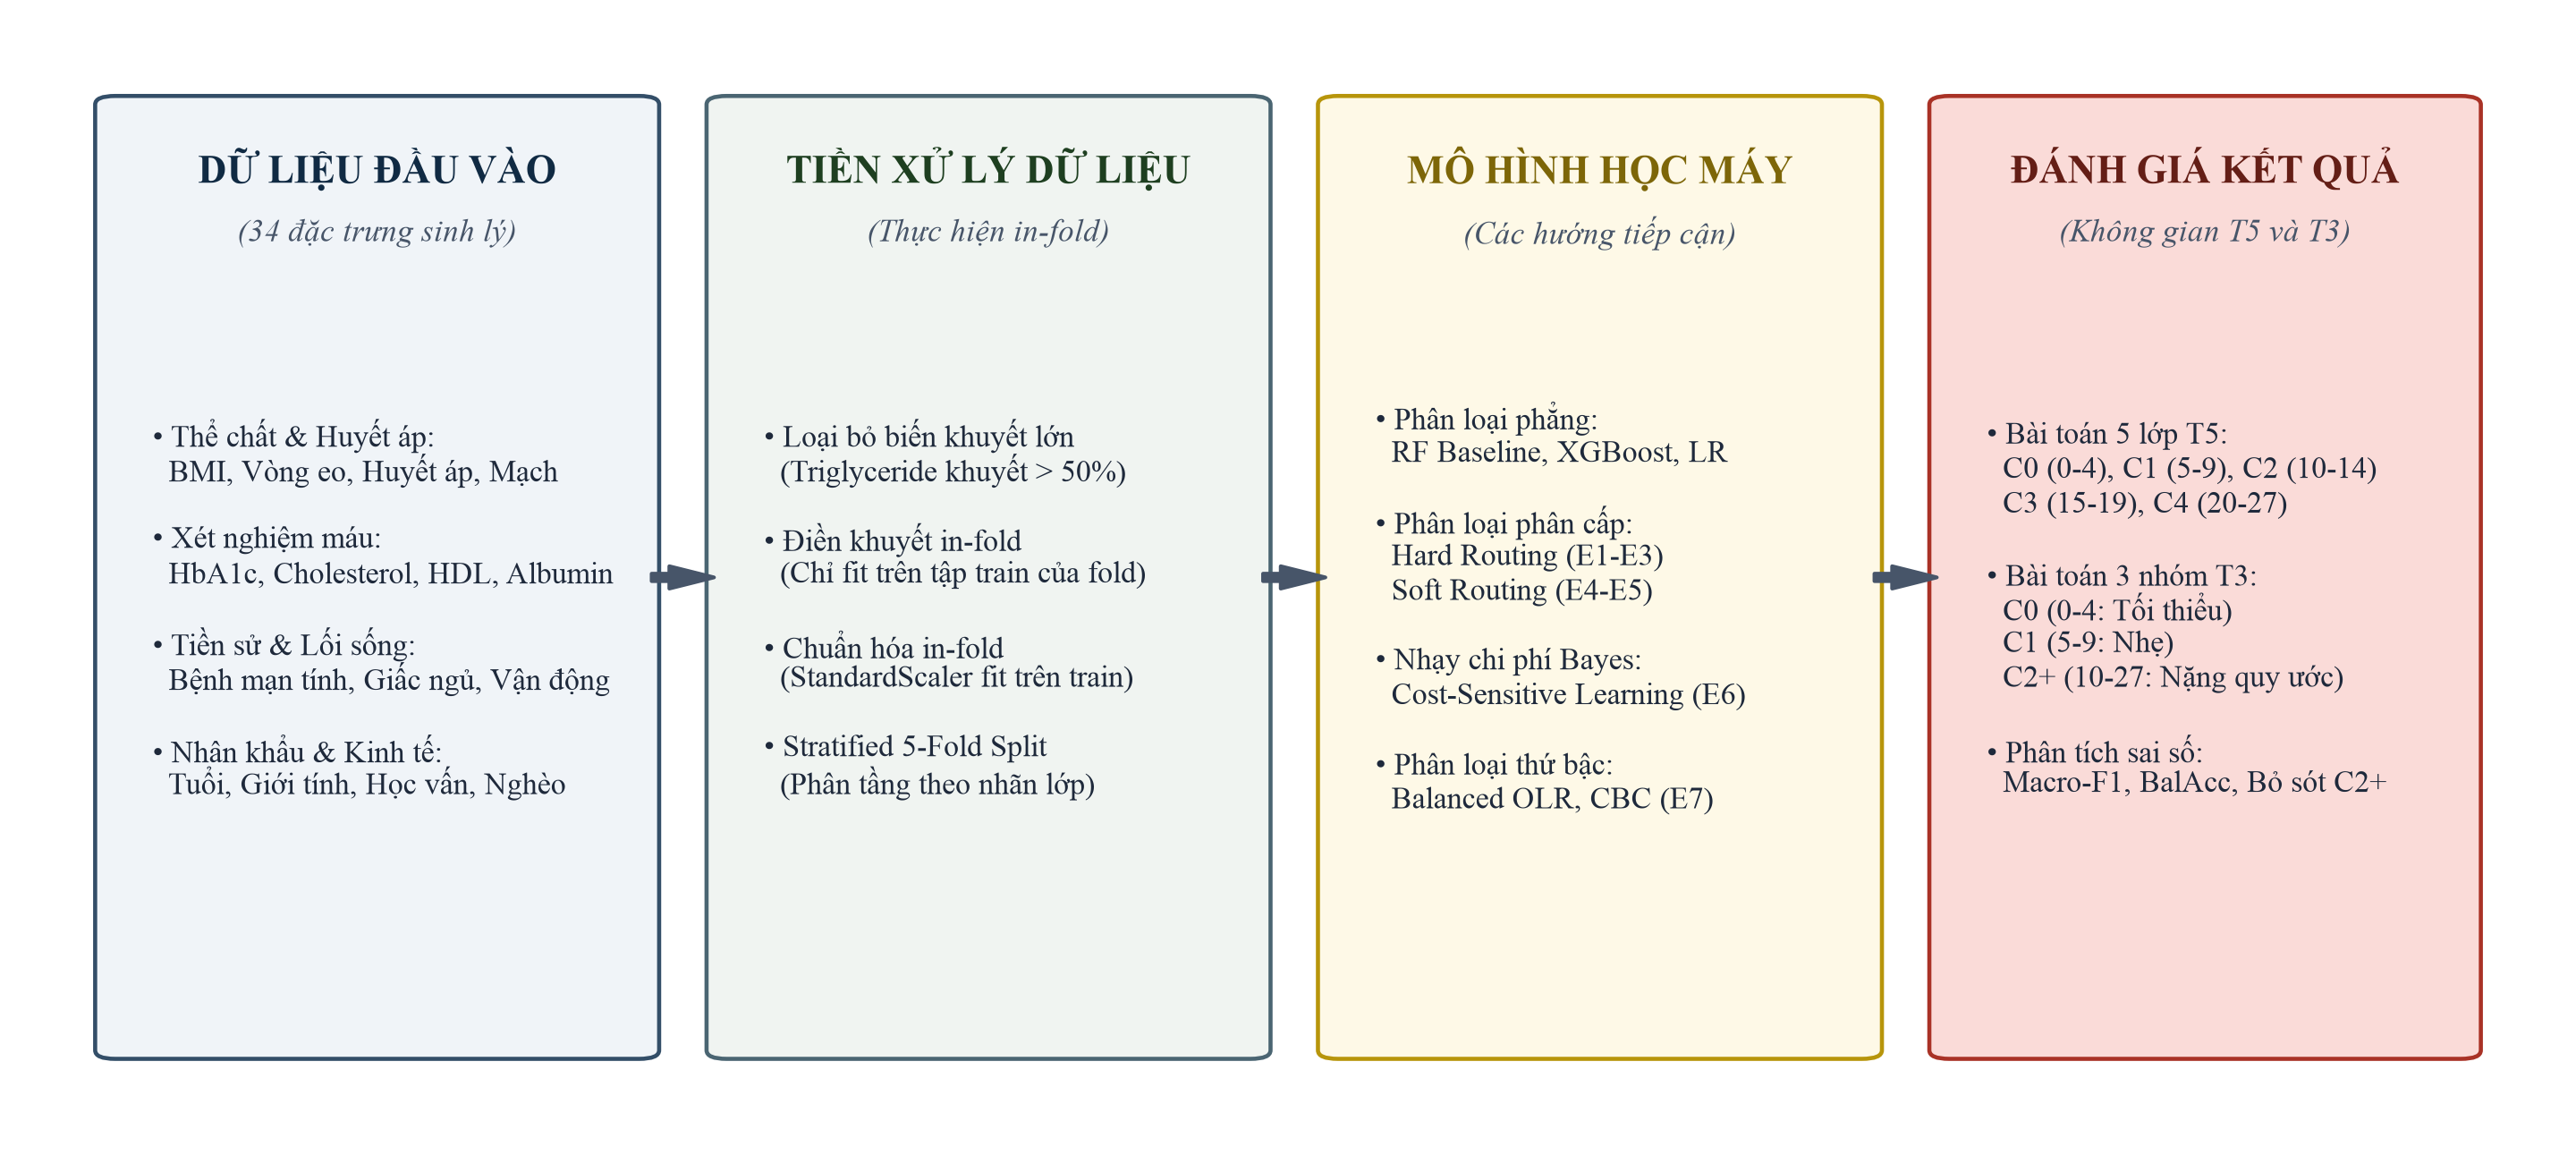
\includegraphics[width=0.92\textwidth]{figures/fig1_problem_formulation.png}
\label{fig:problem-formulation}
\end{figure}

Mục tiêu học máy là tìm kiếm một hàm giả thuyết $f: \mathbb{R}^d \to \{0, \dots, K-1\}$ sao cho tối ưu hóa đồng thời tính chính xác phân loại và độ an toàn lâm sàng, giảm thiểu tối đa các sai số nghiêm trọng như bỏ sót ca có triệu chứng nặng.

\section{Nội dung và mục tiêu nghiên cứu}
\label{sec:muc-tieu-nghien-cuu}

Để làm rõ tiềm năng và ranh giới thực nghiệm của các mô hình học máy trên dữ liệu sinh lý dạng bảng, nghiên cứu tập trung giải quyết các nội dung trọng tâm sau:
\begin{enumerate}
    \item \textit{Khảo sát mức độ đóng góp của từng nhóm biến số:} Đánh giá định lượng ảnh hưởng của các nhóm đặc trưng nhân khẩu học, lối sống, thể chất và sinh hóa máu thông qua quy trình Feature Ablation có kiểm soát, xác định xem việc bổ sung xét nghiệm máu có mang lại sự cải thiện thực sự so với các chỉ số thể chất cơ bản hay không.
    \item \textit{Đánh giá xu hướng suy giảm hiệu năng theo độ phân giải nhãn:} Đo lường sự thay đổi hiệu năng khi chuyển đổi từ bài toán nhị phân đơn giản ($T_2$) sang các bài toán đa mức ($T_3, T_4, T_5$), tìm hiểu nguyên nhân suy giảm thông qua phân tích tương quan và chồng lấn phân phối đặc trưng.
    \item \textit{Xây dựng và so sánh các hướng tiếp cận phân loại trên không gian 3 nhóm ($T_3$):} Triển khai và đối chuẩn 4 trường phái mô hình: phân loại phẳng cơ sở, phân loại phân cấp hai giai đoạn định tuyến cứng, phân loại phân cấp định tuyến mềm kết hợp lý thuyết quyết định nhạy chi phí Bayes, và các mô hình phân loại thứ bậc.
    \item \textit{Định lượng sự đánh đổi lâm sàng và phân tích rủi ro:} Khảo sát sự đánh đổi giữa các chỉ số thống kê (Macro-F1, Balanced Accuracy) với tiêu chí an toàn y tế (số lượng ca trầm cảm nặng bị mô hình phân loại nhầm thành bình thường).
    \item \textit{Kiểm định tính ổn định ngoại suy theo thời gian:} Đánh giá khả năng khái quát hóa của các mô hình trên một chu kỳ khảo sát độc lập sau 2 năm (NHANES 2015--2016) để kiểm chứng khả năng chống chịu hiện tượng trôi phân phối dữ liệu.
\end{enumerate}

\section{Phạm vi và giới hạn nghiên cứu}
\label{sec:pham-vi-nghien-cuu}

Để bảo đảm tính chặt chẽ về mặt phương pháp luận, các giới hạn của đề tài được xác định rõ:
\begin{itemize}
    \item \textit{Dữ liệu nghiên cứu:} Sử dụng dữ liệu khảo sát cộng đồng NHANES của CDC Hoa Kỳ (chu kỳ phát triển 2013--2014 và chu kỳ kiểm định ngoại suy 2015--2016), áp dụng cho người tham gia từ 20 tuổi trở lên có đầy đủ 9 câu hỏi PHQ-9.
    \item \textit{Dạng đặc trưng:} Chỉ khai thác các đặc trưng dạng bảng thu được từ phỏng vấn và khám sức khỏe định kỳ. Đề tài không sử dụng tín hiệu chuỗi thời gian như điện tâm đồ hay điện não đồ.
    \item \textit{Mục đích ứng dụng:} Kết quả dự đoán đóng vai trò công cụ sàng lọc phân tầng rủi ro trong y tế dự phòng cộng đồng, không có chức năng chẩn đoán xác định bệnh học thay thế bác sĩ tâm thần.
\end{itemize}

\section{Phương pháp tiếp cận và cấu trúc báo cáo}
\label{sec:phuong-phap-va-dong-gop}

Nghiên cứu triển khai quy trình thực nghiệm có kiểm soát với hai giai đoạn nối tiếp như minh họa trong Hình \ref{fig:research-progression}:
\begin{enumerate}
    \item \textit{Giai đoạn 1 -- Khảo sát bài toán 5 mức độ gốc ($T_5$):} Thử nghiệm 4 thuật toán học máy phổ biến gồm Logistic Regression, Decision Tree, Random Forest và XGBoost. Qua kiểm định chéo lồng nhau, Random Forest được lựa chọn làm mô hình cơ sở chính cho các bước tiếp theo dựa trên sự cân bằng tốt giữa điểm số Macro-F1 và tính ổn định.
    \item \textit{Giai đoạn 2 -- Khảo sát đa hướng tiếp cận trên không gian 3 nhóm ($T_3$):} Thử nghiệm 12 cấu hình mô hình thuộc 4 trường phái khác nhau ($E_0 \to E_7$), từ phân loại phẳng, phân cấp cứng, phân cấp mềm Bayes đến phân loại thứ bậc.
\end{enumerate}

\begin{figure}[htbp]{Tiến trình nghiên cứu hai giai đoạn từ bài toán $T_5$ sang không gian $T_3$.}
\centering
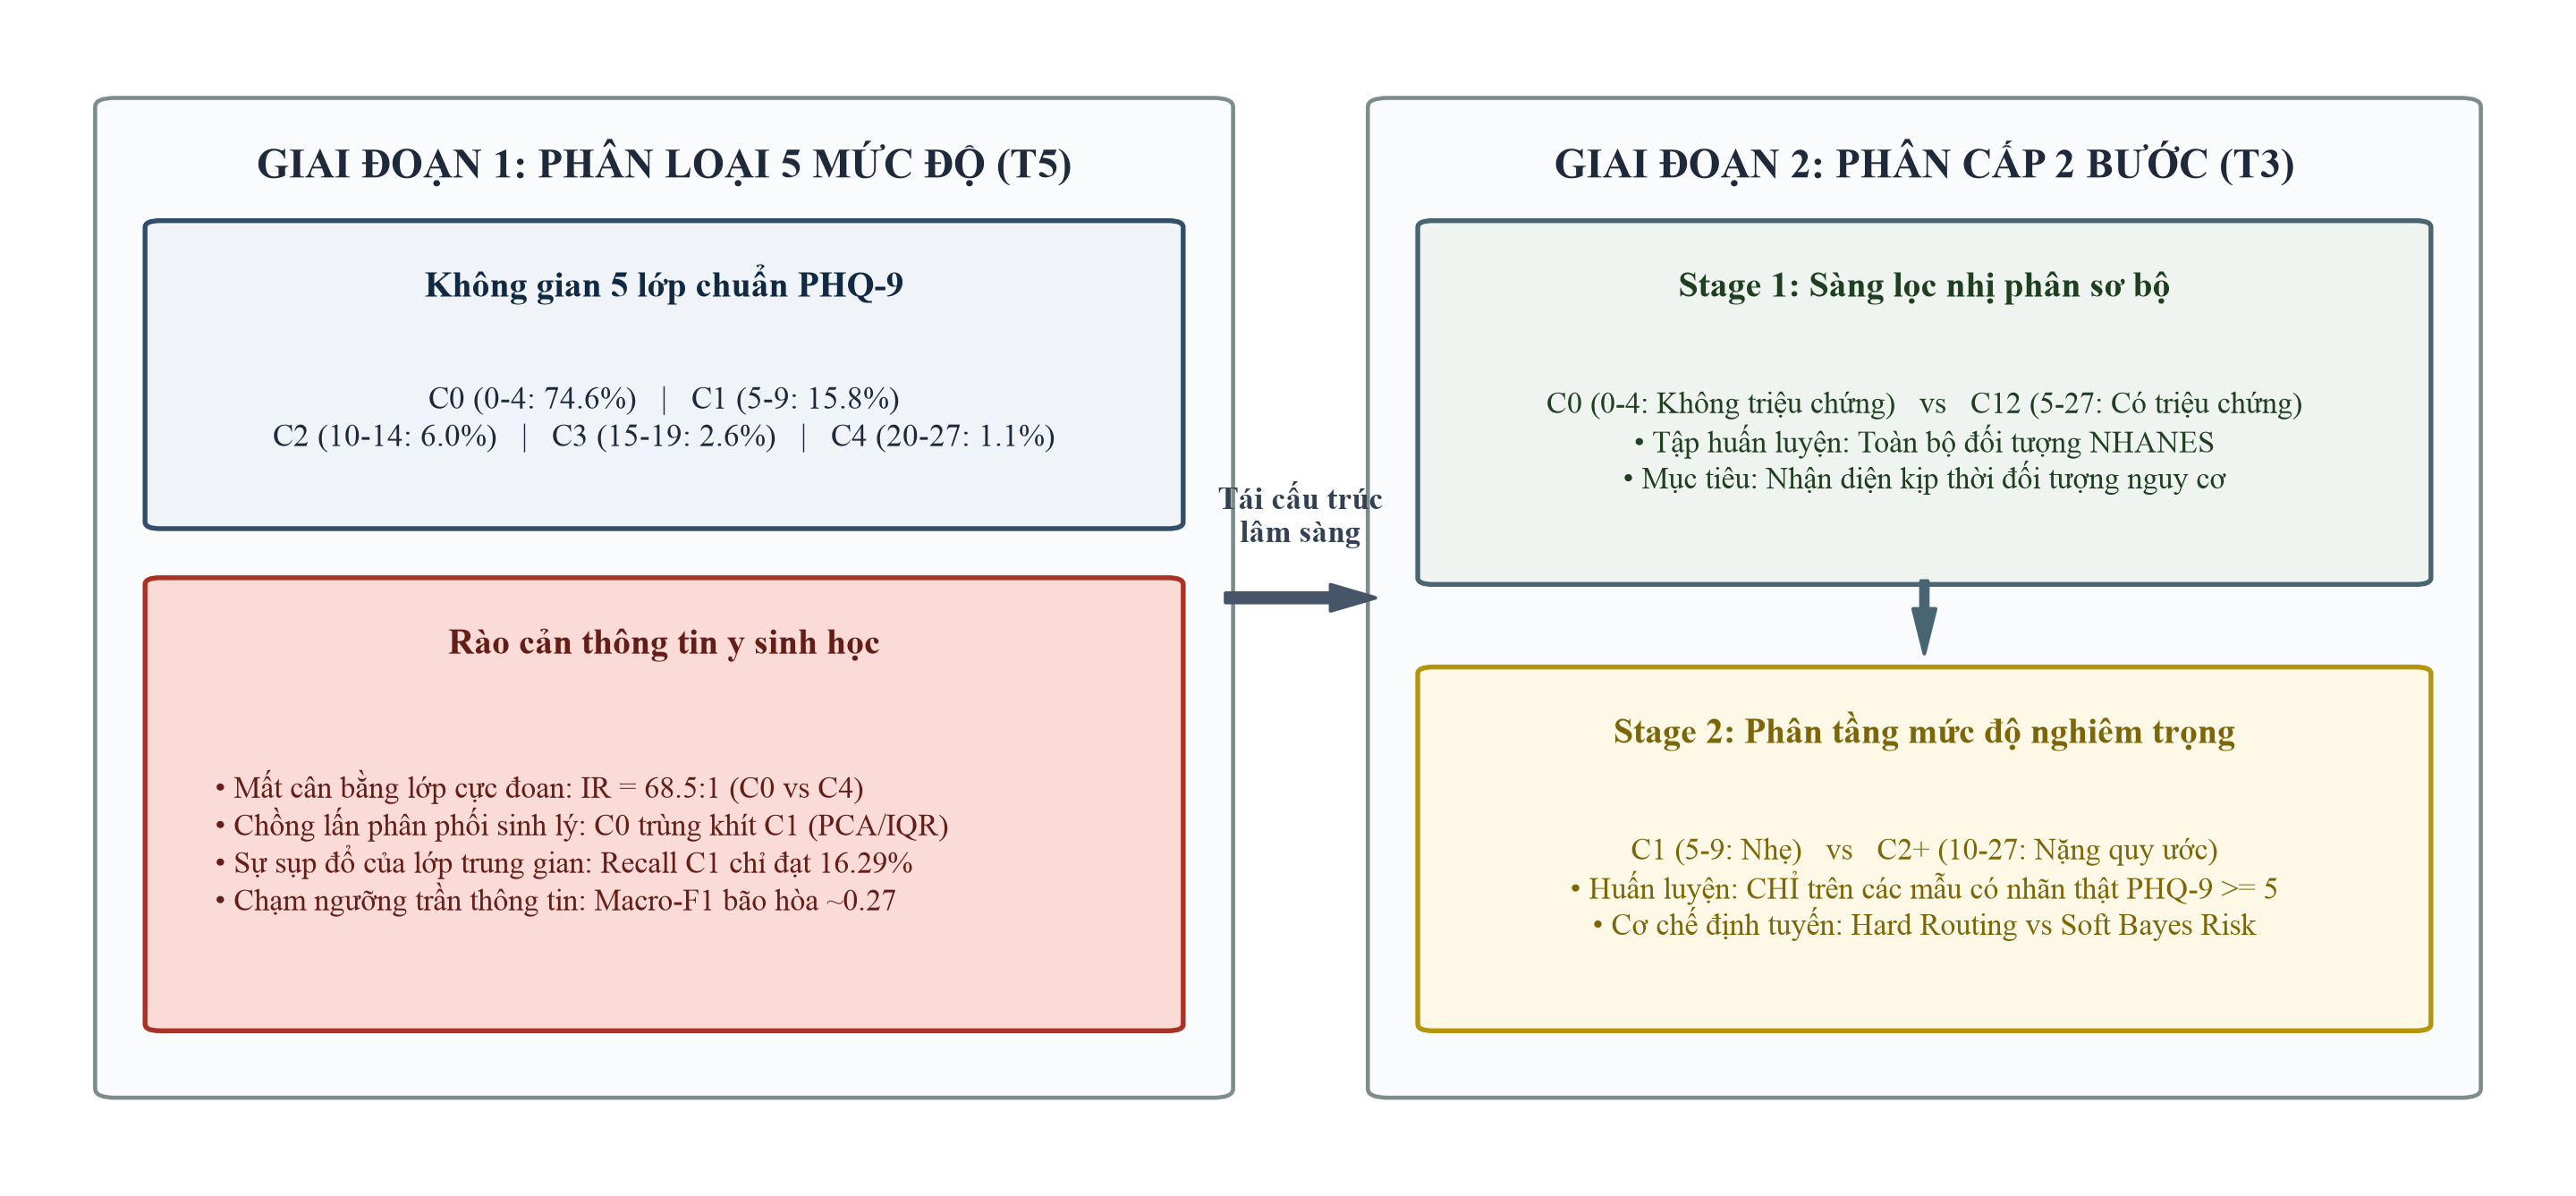
\includegraphics[width=0.92\textwidth]{figures/fig_research_progression_t5_to_t3.png}
\label{fig:research-progression}
\end{figure}

Báo cáo nghiên cứu được bố cục thành 5 chương:
\begin{itemize}
    \item \textit{Chương 1: Giới thiệu} -- Bối cảnh, phát biểu bài toán, mục tiêu nghiên cứu và phạm vi đề tài.
    \item \textit{Chương 2: Cơ sở lý thuyết và các nghiên cứu liên quan} -- Thang đo PHQ-9, đặc thù dữ liệu y tế dạng bảng, các trường phái mô hình hóa và tổng quan y văn liên quan.
    \item \textit{Chương 3: Dữ liệu và phương pháp nghiên cứu} -- Nguồn dữ liệu NHANES, quy trình tiền xử lý in-fold, thiết kế không gian đặc trưng và các kiến trúc mô hình $E_0 \to E_7$.
    \item \textit{Chương 4: Thực nghiệm và thảo luận} -- Kết quả Feature Ablation, so sánh thuật toán cơ sở, suy giảm hiệu năng theo độ chi tiết nhãn, đối sánh các mô hình trên $T_3$, phân tích chi phí Bayes và kiểm định theo thời gian.
    \item \textit{Chương 5: Kết luận và hướng phát triển} -- Tổng kết các phát hiện chính, đóng góp khoa học, phân tích giới hạn của đề tài và đề xuất hướng nghiên cứu tiếp theo.
\end{itemize}
